\begin{figure}[htbp]
\centering
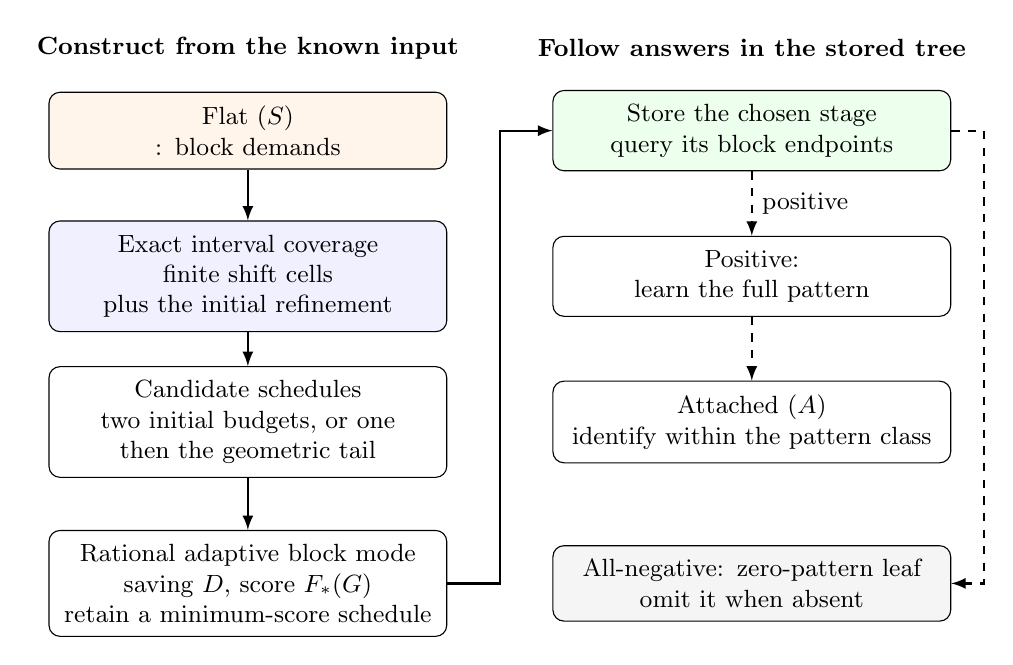
\begin{tikzpicture}[every node/.style={font=\small},
  box/.style={draw,rounded corners,align=center,inner sep=5pt,text width=4.7cm},
  arr/.style={-latex,thick},exec/.style={-latex,thick,dashed}]
  \node[font=\small\bfseries] at (-3.2,1.05) {Construct from the known input};
  \node[font=\small\bfseries] at (3.2,1.05) {Follow answers in the stored tree};
  \node[box,fill=orange!8] (hull) at (-3.2,0)
    {Flat \ExpectedTree$(S)$\\\HullData: block demands};
  \node[box,fill=blue!6] (covers) at (-3.2,-1.85)
    {Exact interval coverage\\finite shift cells\\plus the initial refinement};
  \node[box] (variants) at (-3.2,-3.7)
    {Candidate schedules\\two initial budgets, or one\\then the geometric tail};
  \node[box] (score) at (-3.2,-5.75)
    {Rational adaptive block mode\\saving $D$, score $F_*(G)$\\retain a minimum-score schedule};
  \node[box,fill=green!7] (stored) at (3.2,0)
    {Store the chosen stage\\query its block endpoints};
  \node[box] (positive) at (3.2,-1.85)
    {Positive: \EndpointCode\\learn the full pattern};
  \node[box] (child) at (3.2,-3.7)
    {Attached \ExpectedTree$(A)$\\identify within the pattern class};
  \node[box,fill=gray!8] (zero) at (3.2,-5.75)
    {All-negative: zero-pattern leaf\\omit it when absent};
  \draw[arr] (hull) -- (covers);
  \draw[arr] (covers) -- (variants);
  \draw[arr] (variants) -- (score);
  \draw[arr] (score.east) -- (0,-5.75) -- (0,0) -- (stored.west);
  \draw[exec] (stored) -- node[right]{positive} (positive);
  \draw[exec] (positive) -- (child);
  \draw[exec] (stored.east) -- (6.15,0) -- (6.15,-5.75)
    -- (zero.east);
\end{tikzpicture}
\caption{The polynomial expected-depth algorithm first computes hull
patterns and their block demands, then uses interval coverage to build
candidate schedules and selects one by its rational score. Solid arrows
show this construction-time data flow, using the supplied incidence
table and prior. The chosen stage is then stored as a query tree: dashed
arrows trace the unknown hypothesis through discovery, endpoint
decoding, and its already constructed recursive child. The adaptive
mode decides whether discovery stops at the first positive endpoint or
queries both endpoints. The algorithm makes this schedule choice
deterministically; the certificate's mixture is used to prove its cost
bound.}
\label{fig:expected-procedure-flow}
\end{figure}

